\subsubsection{Измерения}
1. Для начала измерены или изучены в паспорте некоторые
величны:
\begin{itemize}
    \item толщина проволоки $\delta = 0.46$ мм,
    \item длина проволоки $l = 177$ см,
    \item расстояние от зеркала до линейки $d = 142$ см,
    \item длина штанги $r = 15$ см.
\end{itemize}

2. Для разных масс измерены отклонения 4 раза, результаты
приведены в таблице (цифры в первой строчке -- номер измерения).
\begin{center}

\begin{tabular*}{0.75\textwidth}{@{\extracolsep{\fill}}|c|c|c|c|c|}
    \hline
    Вес, г & 1, см & 2, см & 3, см & 4, см \\
    \hline
    501.4 & 16.0 & 16.7 & 17.0 & 16.9\\
    \hline
    747.0 & 19.1 & 19.6 & 19.7 & 19.9\\
    \hline
    993.1 & 21.9 & 22.5 & 22.5 & 22.4\\
    \hline
    1238.7 & 24.5 & 25.0 & 25.3 & 25.4\\
    \hline
    1484.2 & 27.1 & 27.8 & 27.9 & 28.0\\
    \hline
    1729.8 & 29.7 & 30.3 & 30.4 & 30.5\\
    \hline
    1975.1 & 32.4 & 32.8 & 33.0 & 33.1\\
    \hline
    2220.4 & 34.8 & 35.3 & 35.6 & 35.5\\
    \hline
    2465.9 & 37.3 & 37.7 & 38.0 & 38.0\\
    \hline
    2711.7 & 39.7 & 40.1 & 40.5 & 40.5\\
    \hline
    2957.3 & 42.6 & 42.6 & 42.4 & 43.0\\
    \hline
    3201.7 & 44.8 & 44.8 & 44.9 & 44.9\\
    \hline

\end{tabular*}

\end{center}

\subsubsection{Обработка}
3. Получим формулу для расчета удлинения пружины:
\begin{equation}
    \Delta x = \frac{\Delta l\cdot r}{2d}.
\end{equation}

4. Второй закон Ньютона для грузов:
\begin{equation}
    k\Delta x = mg + F.
\end{equation}

5. Модуль Юнга, объединяя (12) и (13):
\begin{equation}
    E = k\frac lS = \frac{mgl}{S\Delta x} = \frac{2mgld}{S\Delta lr}.
\end{equation}
6. Построим график $m = k\Delta l + m_0$, где $m_0$
определяется начальными условиями (масса проволоки):
\begin{figure}[H]
    \centering
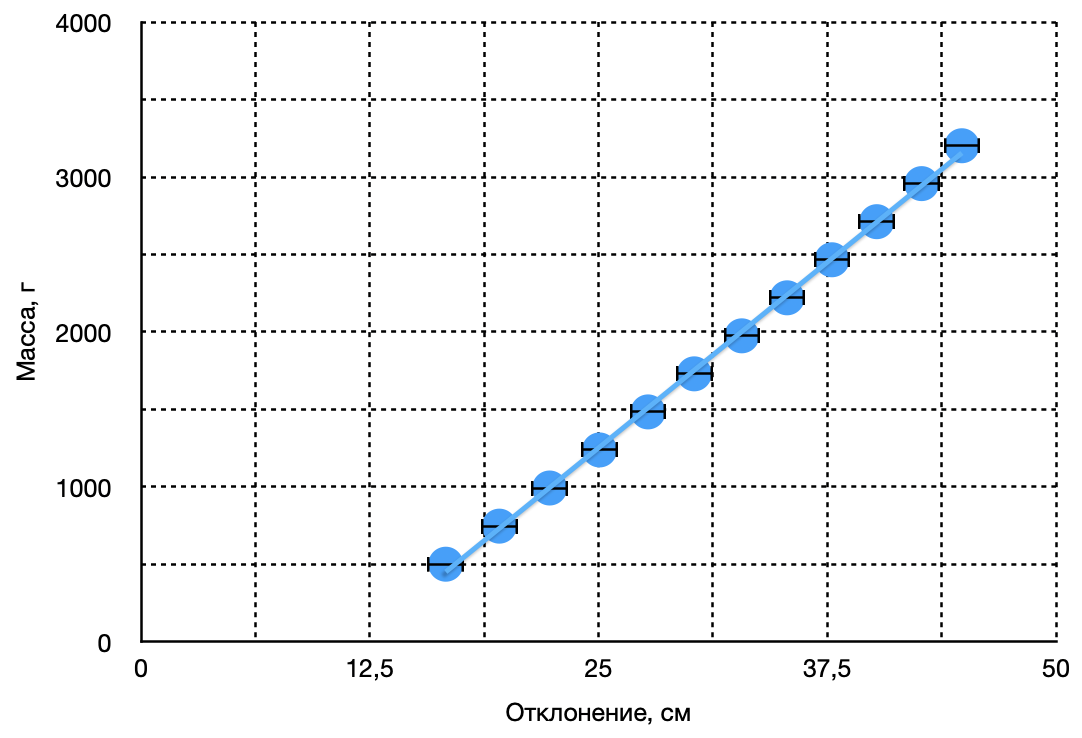
\includegraphics[width=0.75\linewidth,center]{p6.png}
    \label{fig:my_label}
\end{figure}
По графику $k = (9.6 \pm 0.6)$ кг/м.

7. Выразим E:
\begin{center}
$E = \frac{2kgld}{Sr} = 1.90 \cdot 10^{10} \pm 1.2 \cdot 10^9$ Па.
\end{center}
